% -*- mode: latex; -*- mustache tags:  
\documentclass[10pt,twoside,english]{_support/latex/sbabook/sbabook}
\let\wholebook=\relax

\usepackage{import}
\subimport{_support/latex/}{common.tex}

%=================================================================
% Debug packages for page layout and overfull lines
% Remove the showtrims document option before printing
\ifshowtrims
  \usepackage{showframe}
  \usepackage[color=magenta,width=5mm]{_support/latex/overcolored}
\fi


% =================================================================
\title{Learning Object-Oriented Programming, Design and TDD with Pharo}
\author{Stéphane Ducasse}
\series{The Pharo TextBook Collection}

\hypersetup{
  pdftitle = {Learning Object-Oriented Programming, Design and TDD with Pharo},
  pdfauthor = {Stéphane Ducasse},
  pdfkeywords = {Introduction, programming, design, testing, Pharo, Smalltalk}
}


% =================================================================
\begin{document}

% Title page and colophon on verso
\maketitle
\pagestyle{titlingpage}
\thispagestyle{titlingpage} % \pagestyle does not work on the first one…

\cleartoverso
{\small

  Copyright 2017 by Stéphane Ducasse.

  The contents of this book are protected under the Creative Commons
  Attribution-ShareAlike 3.0 Unported license.

  You are \textbf{free}:
  \begin{itemize}
  \item to \textbf{Share}: to copy, distribute and transmit the work,
  \item to \textbf{Remix}: to adapt the work,
  \end{itemize}

  Under the following conditions:
  \begin{description}
  \item[Attribution.] You must attribute the work in the manner specified by the
    author or licensor (but not in any way that suggests that they endorse you
    or your use of the work).
  \item[Share Alike.] If you alter, transform, or build upon this work, you may
    distribute the resulting work only under the same, similar or a compatible
    license.
  \end{description}

  For any reuse or distribution, you must make clear to others the
  license terms of this work. The best way to do this is with a link to
  this web page: \\
  \url{http://creativecommons.org/licenses/by-sa/3.0/}

  Any of the above conditions can be waived if you get permission from
  the copyright holder. Nothing in this license impairs or restricts the
  author's moral rights.

  \begin{center}
    
\includegraphics[width=0.2\textwidth]{_support/latex/sbabook/CreativeCommons-BY-SA.pdf}
  \end{center}

  Your fair dealing and other rights are in no way affected by the
  above. This is a human-readable summary of the Legal Code (the full
  license): \\
  \url{http://creativecommons.org/licenses/by-sa/3.0/legalcode}

  \vfill

  % Publication info would go here (publisher, ISBN, cover design…)
  Layout and typography based on the \textcode{sbabook} \LaTeX{} class by Damien
  Pollet.
}


\frontmatter
\pagestyle{plain}

\tableofcontents*
\clearpage\listoffigures

\mainmatter

\chapter{Objects and classes}\label{cha_objects}
Pharo is a pure object-oriented programming language, i.e., everything in the system is an object i.e., an entity created by a class and reacting to messages. In this chapter you will learn the concepts of object-oriented programming: \textit{objects} and \textit{classes}. 

Objects are entities that communicate via messages and react to messages by executing certain tasks. Moreover objects hide the way they define these tasks: the client of an object send a message to an object and the system find the corresponding method to be executed. Messages specify what should be done and methods how it should be done. 

Objects are created by classes that are object factories: Classes define the structure and behavior of objects (in terms of methods) but each object has a specific state and identity that is unique and different from all other objects. A class defines methods that specify how a message is actually implemented. 
\section{Objects: Entities reacting to messages}
In chapter \ref{cha:PlayingWithObjects} you created objects and sent them messages without really paying attention because this is natural. Let us analyze what we did and understand the first principle behind objects. As you saw, you created objects, turtles but also numbers and colors and sent them messages. In reaction to these messages, objects performed some actions. For example, a turtle knows how to change its direction, to move forward and so on.

An object is a computer entity that once created receives messages and performs some actions in reaction. An object \textit{executes} a \textit{method} in response to a message reception as shown in Figure . A method is just a sequence of instructions i.e., assignments, messages to other objects, that has a name and whose name can be used in a message to ask for the method execution. 
\subsection{Message: the what should be executed}
The message \textcode{square:} is send to a new turtle with 100 as argument. The message expresses what the receiver should do. 

\begin{displaycode}{plain}
Turtle new square: 100
\end{displaycode}
\subsection{Method: the how we execute it}
The method definition \textcode{square:} below defines step by step what are the actions to be done in response to the message \textcode{square:}. We will show later how the mapping between a message and a method is done at runtime. 

\begin{displaycode}{plain}
square: size
	4 timesRepeat: [ self go: size; turn: 90 ]
\end{displaycode}

\begin{important}
A message represents \textit{what} the object can do, while a method specifies \textit{how} the behavior is realized. 
\end{important}

An object can also send messages to other objects. For example, when a turtle draws a line it send messages to an object representing the line  color and send messages numbers.


\begin{figure}

\begin{center}
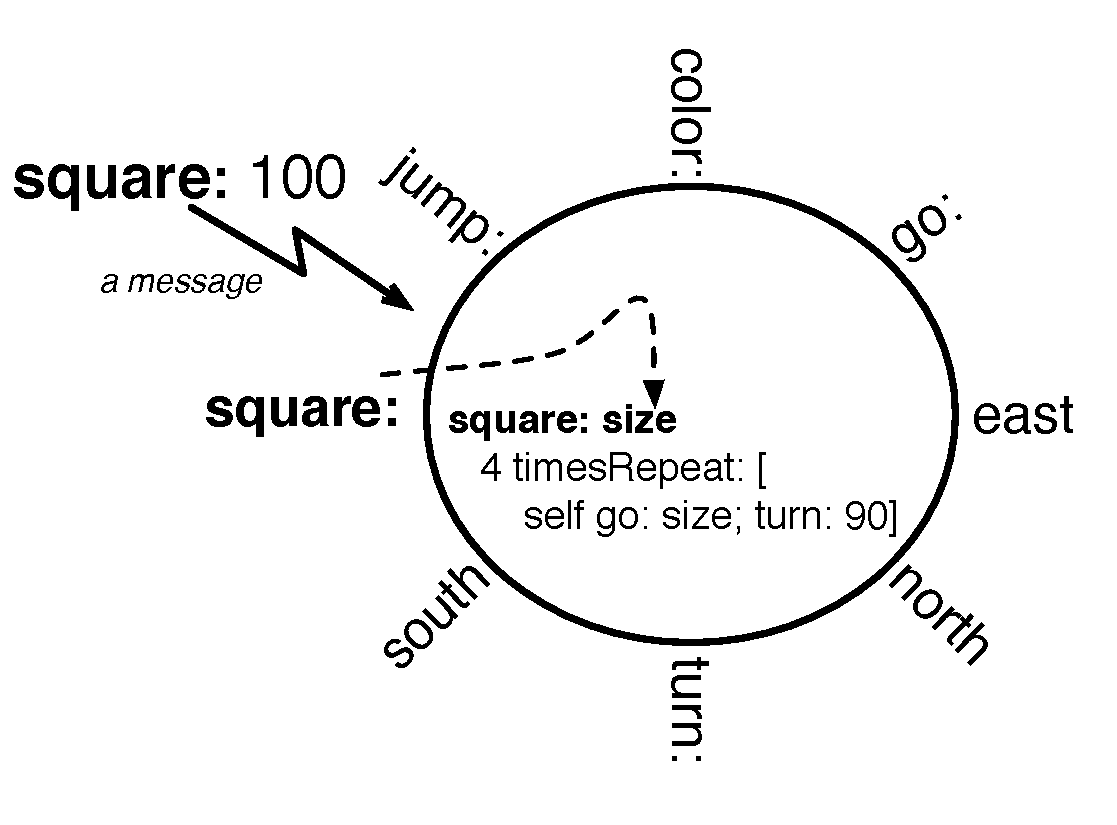
\includegraphics[width=0.5\textwidth]{/Users/ducasse/Workspace/FirstCircle/MyBooks/Bk-Writing/PharoBooks/LearningOOPWithPharoTrans/_result/pdf/Chapters/ObjectsAndClasses/figures/basicMessageMethod.pdf}\caption{An object presents to the other objects an interface composed of a set of messages defining \textit{what} he can do. This behavior is realized by methods that specify \textit{how} the behavior is implemented. When a message is sent to an object a method with the message name is looked up and executed. \label{basicMessageMethod}}\end{center}
\end{figure}


\begin{important}
An object is an entity that once created receives messages and performs some actions in reaction. When a message is sent to an object, a method with the message name is looked up and executed.
\end{important}
\section{An object has  a unique identity}
An object has an identity. Each object is unique and is uniquely identifiable. In Pharo, the message == allows one to test object identity as shown by the following examples.

First we create two different turtles and referred to them using the variables \textcode{caro} and \textcode{marg}. As they are different objects the test returns false.

\begin{displaycode}{plain}
| caro marg |
caro := Turtle new.
marg := Turtle new.
caro == marg
>>> false
\end{displaycode}

We create only one turtle and assign it to the variable \textcode{caro}. We compare what is pointed by the variable \textcode{caro} and obvisouly this is the same object, so the test is true.

\begin{displaycode}{plain}
| caro marg |
caro := Turtle new.
caro == caro
>>>  true
\end{displaycode}

Here we create only one object but refer to it by two different variables. However this is not changing anything because the two variables refer to the same object that has the same identity so we get \textcode{true} meaning that the identity of the object pointed by \textcode{caro} is the same than the one pointed by \textcode{marg}.

\begin{displaycode}{plain}
| caro marg |
caro := Turtle new.
marg := caro.
caro == marg
>>> true
\end{displaycode}

\begin{important}
An object has an unique identity.
\end{important}
\section{An object is a protective entity}
An object is responsible of the way it realizes its reaction to a
message.  It \textit{offers services} but \textit{hides} the way they are implemented (see Figure \ref{fig:encapsulationAtWork}). We do not have to know how the method associated with the message selector is implemented.  Only the object knows the exact definition of the method.  This is when we define the method \textcode{square:} that defines how a turtle draws a square of a given size, that we focus on \textit{how} a turtle draws a square. Figure \ref{fig:encapsulationAtWork} shows the message and the method \textcode{square:}. The method \textcode{square:} defines how to draw step by step a square, however the object only offers the message square: and does not show it implementation.

\begin{important}
An object presents to the other objects an interface composed of a set of messages defining \textit{what} the object can do. This behavior is realized by methods that specify \textit{how} the behavior is implemented. To perform something useful data are most of the time required. Data are only accessed by the methods.
\end{important}

\begin{important}
An object is responsible of the way it realizes its reaction to a message. It offers services and hides the way they are implemented.
\end{important}

From a turtle \textit{user} point of view, the only relevant information is that the turtle effectively receiving the message \textcode{square:} executes the method that draws a square. So changing the definition of the \textcode{square:} method  to the one below does not have any consequence on the methods that call it. Figure \ref{fig:encapsulationAtWork2} illustrates this point.

\begin{displaycode}{plain}
square: s
   "Make the receiver draw a square of size s"

   self go: s; turn: 90; go: s; turn: 90.
   self go: s; turn: 90; go: s; turn: 90
\end{displaycode}


\begin{figure}

\begin{center}
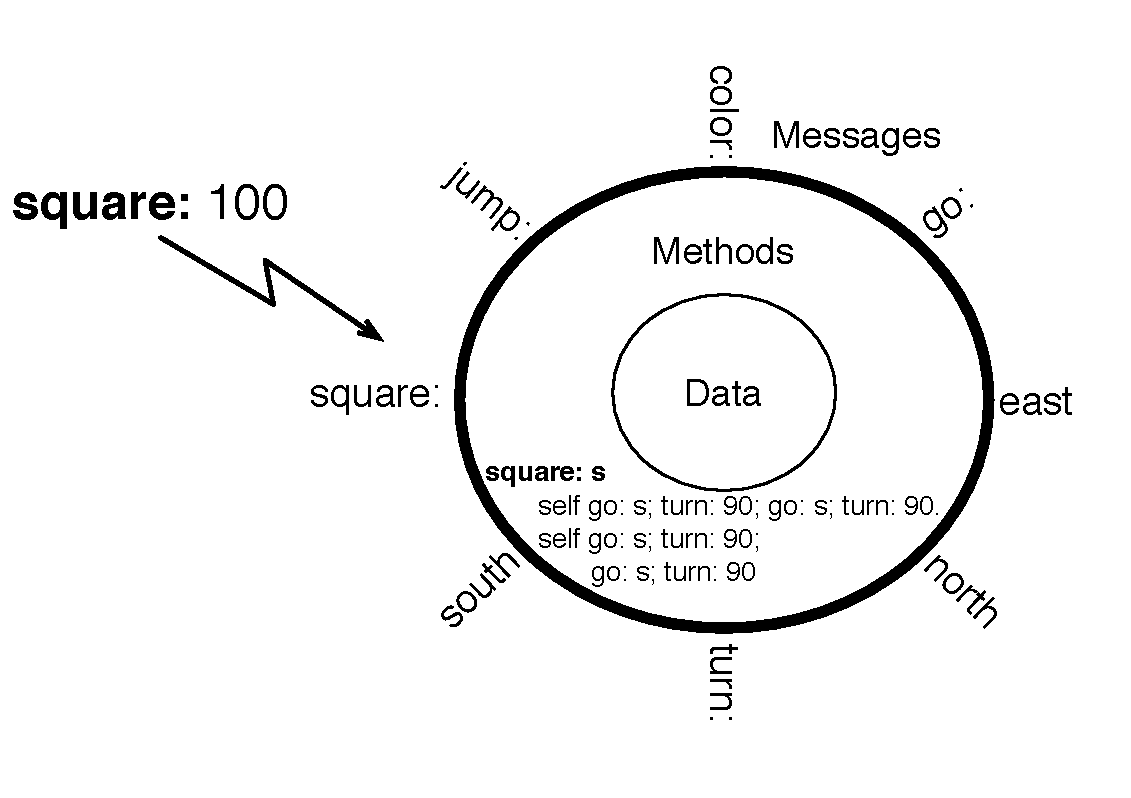
\includegraphics[width=0.45\textwidth]{/Users/ducasse/Workspace/FirstCircle/MyBooks/Bk-Writing/PharoBooks/LearningOOPWithPharoTrans/_result/pdf/Chapters/ObjectsAndClasses/figures/encapsulationAtWork2.pdf}\caption{The message \textcode{square:} can be implemented differently this does not impact the sender of the message who is not concerned by the internals of the object.\label{fig:encapsulationAtWork2}}\end{center}
\end{figure}


Hiding the internal representation is not limited to object-oriented programming but it is central to object-oriented programming. 
\section{An object protects its data}
An object holds some \textit{private data} that represents its state (see Figure \ref{fig:objectOne}). Moreover, it controls its state and should not let other objects play directly with them because this could let him into an inconsistent state.  For example, you do not want to somebody else plays with the data of your bank account directly and really want to control your transaction. 

For example, a turtle can be represented by a position, a direction and a way to indicate if its pen is up or down. But, we cannot directly access these data and change them. For that we have to use the set of messages proposed by a turtle. These methods constitute the \textit{interface} of an object. We say that the object state is \textit{encapsulated}, this means that not everybody can access it. In fact, object-oriented programming is based on encapsulation, i.e., the fact that per default objects are the only ones that can access their own state.


\begin{figure}

\begin{center}
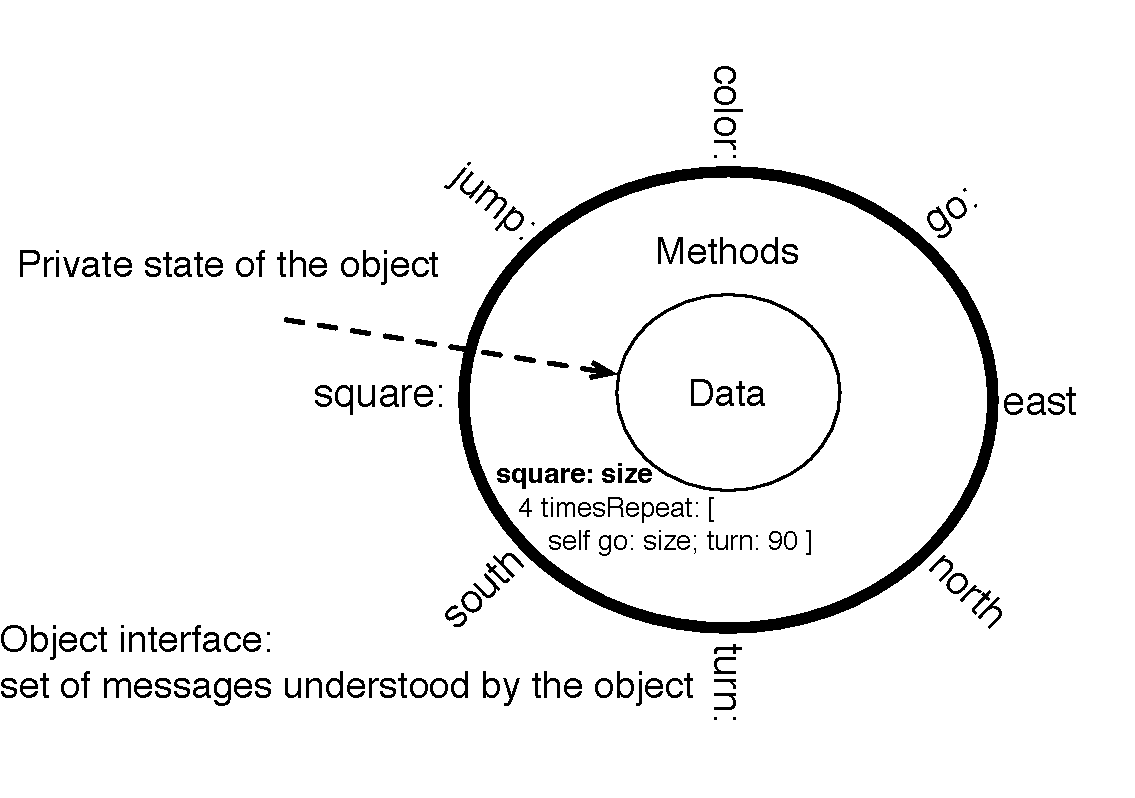
\includegraphics[width=0.45\textwidth]{/Users/ducasse/Workspace/FirstCircle/MyBooks/Bk-Writing/PharoBooks/LearningOOPWithPharoTrans/_result/pdf/Chapters/ObjectsAndClasses/figures/privateData.pdf}\caption{A turtle is an object which has an interface, i.e., a set of messages to which it can reply and a private state that only its methods can access.\label{fig:objectOne}}\end{center}
\end{figure}


In Pharo, a client cannot access the state of an object if the object does not define a method to access it.  Moreover, clients should not  rely on the internal representation of an object because an object is free to change the way it  implements its behavior. Exposing the internal state of an object by defining methods providing access to the object data weakens the control that an object has over its own state.

Our turtle (contrarily to the original Logo turtle) does not provide a way to change directly the status of its pen. The messages \textcode{jump} and \textcode{go} are actually changing the status of the turtle's pen and its position.   


\begin{figure}

\begin{center}
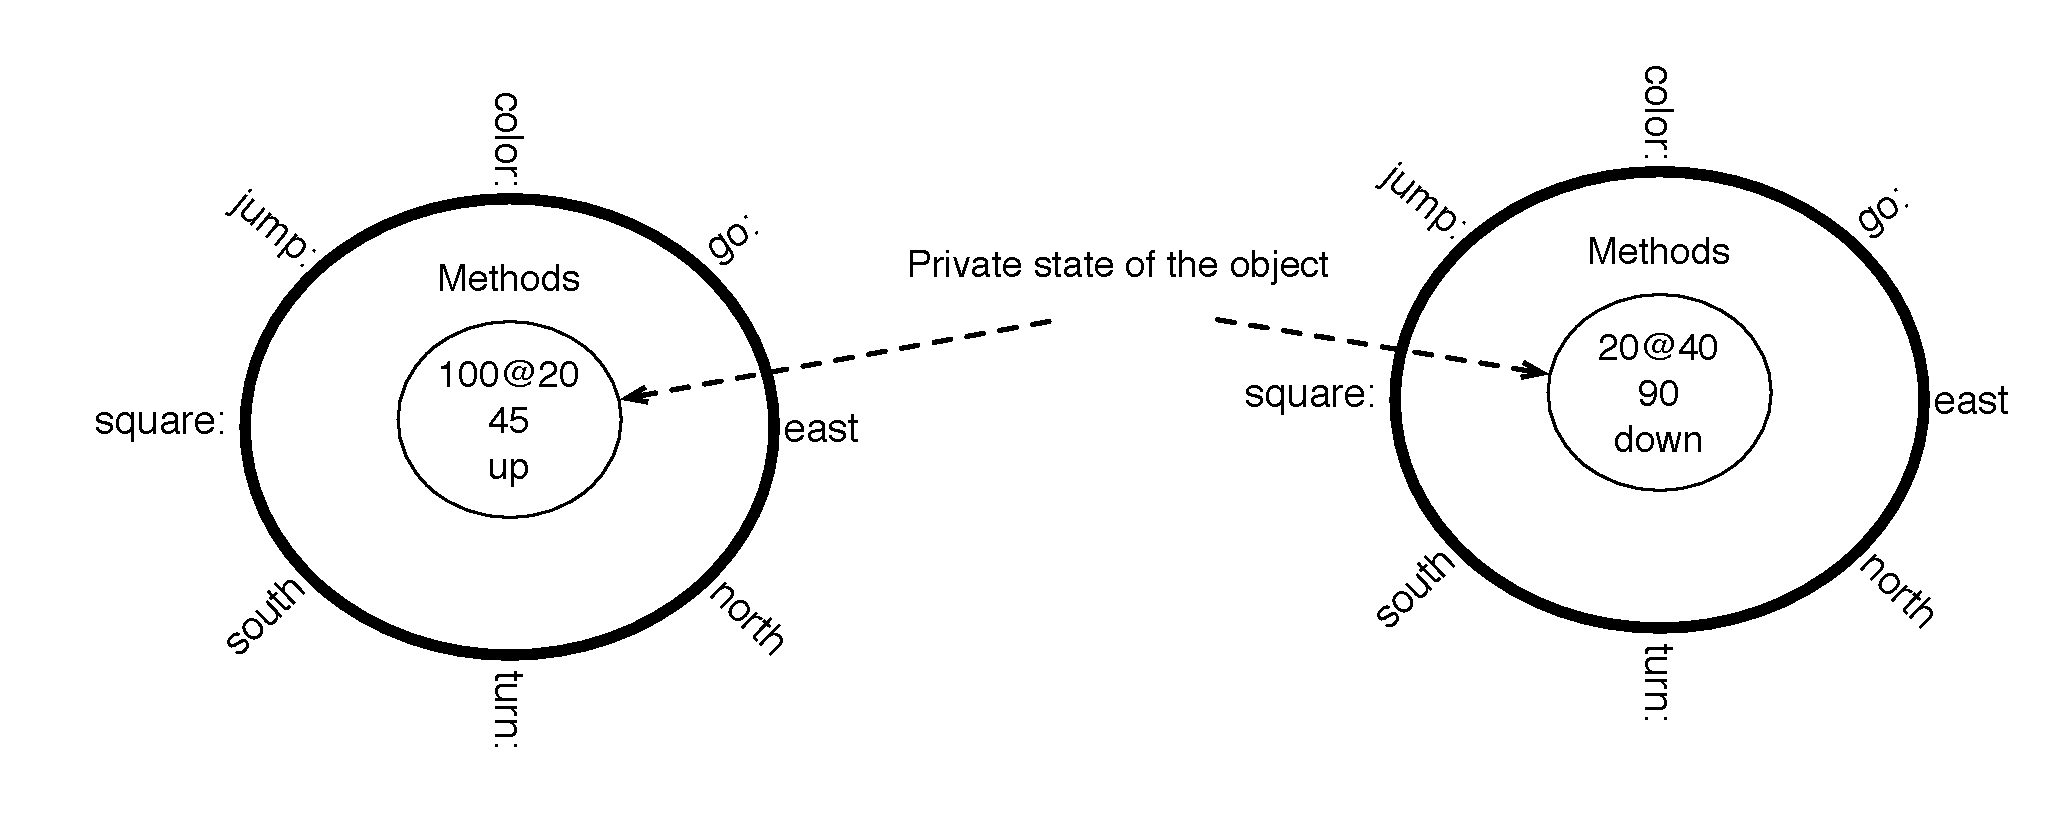
\includegraphics[width=0.7\textwidth]{/Users/ducasse/Workspace/FirstCircle/MyBooks/Bk-Writing/PharoBooks/LearningOOPWithPharoTrans/_result/pdf/Chapters/ObjectsAndClasses/figures/privateDataTwoInstances.pdf}\caption{Two turtles have the same interface, i.e., set of messages  being understood but they have \textit{different} private state representing their  direction, position and pen status.\label{fig:twoInstances}}\end{center}
\end{figure}


\begin{important}
An object holds some \textit{private} data that represents its \textit{internal} state. Each object has its own state. Two objects of the same class shares the same \textit{interface} but have their own private state.
\end{important}
\subsubsection{About behavior}
Behaviour should be associated with the objects responsible for the associated state.
Avoid defining behaviour for which another object is responsible
\section{Some related concepts (to massage)}
\begin{itemize}
\item Abstraction means that we ignore irrelevant details, for example, we abstract from the details of a Shape object and just use its interface (i.e., its operations).
\item Information hiding means that we hide (forbid access to) the representation behind an abstraction, for example, you may not directly access the state of a Shape but must access it only through its interface.
\end{itemize}

 Information hiding: a component should provide all and only the information that the user needs to effectively use it.
Information hiding protects both the provider and the client from changes in the implementation

\begin{itemize}
\item Encapsulation means that related entities are bundled together, for example, a Shape object encapsulates data and related operations for shapes.
\end{itemize}

\textit{Clients should depend only on an interface, so changes to the implementation do not affect them.
Conversely, the provider is free to change the implementation if it knows that clients will not be affected.
Information hiding is important for many reasons — it is a version of the “need to know” principle.
Separate development of components is also enabled if dependencies are restricted to interfaces.}
David L. Parnas. On the Criteria To Be Used in Decomposing Systems into Modules. In CACM 15(12) p. 1053—1058, December 1972.

These three concepts are closely related, but clearly different.

\begin{itemize}
\item Composition refers to the fact that we can compose complex objects from simpler ones. A Picture may be composed of many shapes.
\item Distribution of Responsibility means that we break complex tasks into simpler ones, and handle them at the appropriate level of abstraction, and close to where the relevant knowledge is. If you need to resize a shape object, that task should be handled by the shape itself.
\item Message Passing refers to the idea that you do not “apply procedures to objects”, but that you politely ask them to do something by sending them a message. The object itself then decides whether it has a method to handle that message.
\end{itemize}
\section{Collaborators}
An object is not an isolated entity. It interacts with other objects: Its performs tasks on reaction to message but it also can delegate some subtasks other objects. An object has \textit{collaborators}. A turtle collaborates with points, color, pen but also a graphical canvas on which it draw with its pen. 


\begin{figure}

\begin{center}
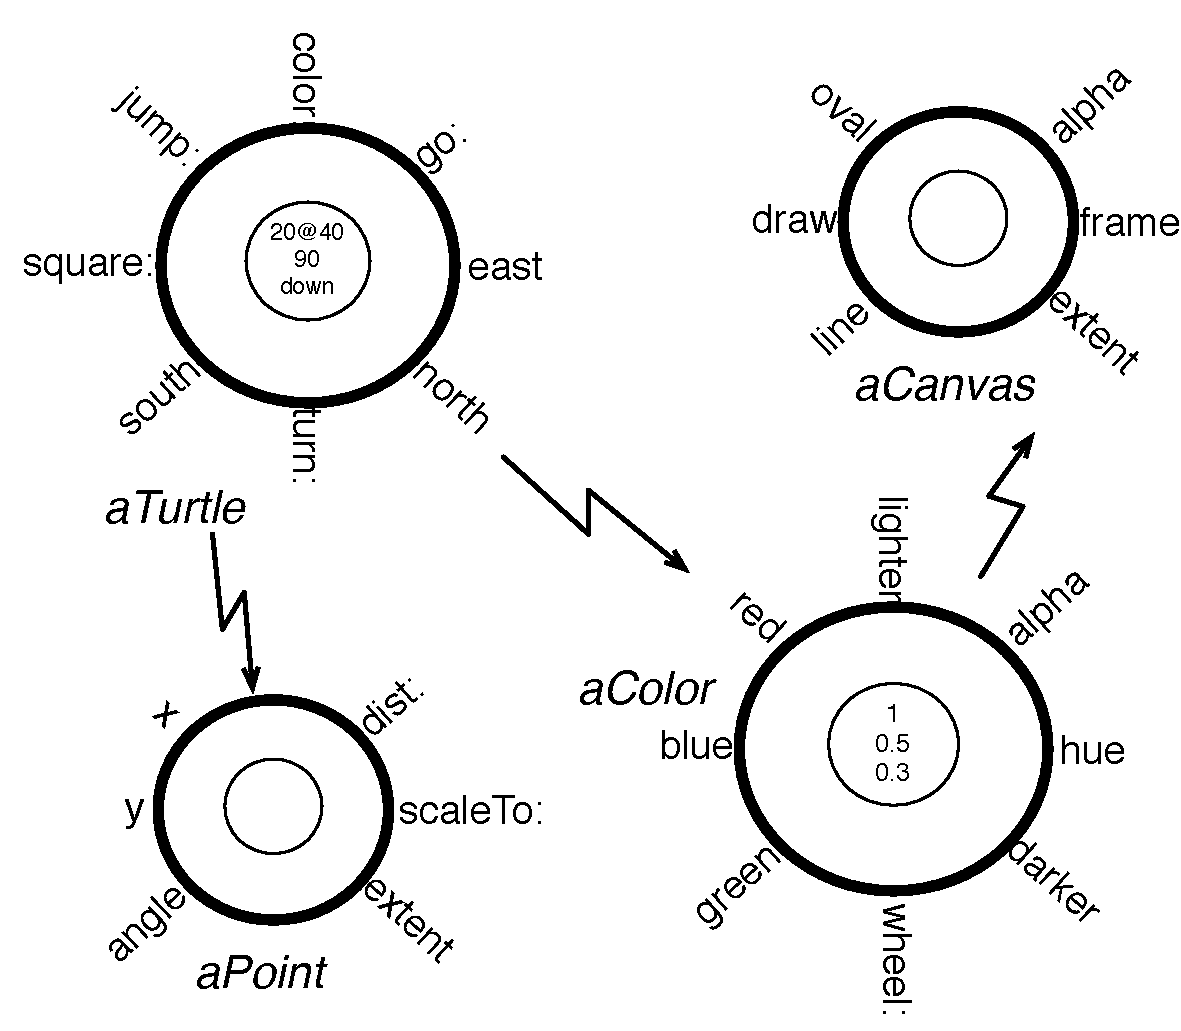
\includegraphics[width=0.7\textwidth]{/Users/ducasse/Workspace/FirstCircle/MyBooks/Bk-Writing/PharoBooks/LearningOOPWithPharoTrans/_result/pdf/Chapters/ObjectsAndClasses/figures/collaborators.pdf}\caption{An object interact with others: either to perform tasks or to request tasks.\label{fig:collaborators}}\end{center}
\end{figure}

\section{Classes: Factoring behavior of similar objects}
As we already saw several turtles can be created independently one of each others.  In the following script two \textcode{Turtle} objects \textcode{caro} and \textcode{marg} execute the method named \textcode{jump}. As a result they change \textit{their respective} position.

\begin{listing}[float]{plain}{Two turtles understanding the same messages}
| caro marg | 
caro := Turtle new.
marg := Turtle new.
caro east. 
marg jump: 100.
caro jump: 100.
marg jump: 200. 
\end{listing}

To avoid duplication of object behavior definition in all similar objects, class-based object-oriented languages introduce the notion of \textit{class}. All the behavior understood by \textcode{caro} and \textcode{marg} is defined in the class \textcode{Turtle} and as such \textit{shared} among all the class objects.  All the turtles share the same method \textcode{jump}. Hence, every time we define a new method in the class \textcode{Turtle}, all the turtles can execute it in response to the corresponding message.

\begin{important}
All objects of the same class share the same behavior, i.e., the same method definitions.
\end{important}
\section{Classes: Factory of objects}
A class is a \textit{factory} of objects, called its \textit{instances}. \textcode{marg} and \textcode{caro} are instances of the class \textcode{Turtle}.
In Pharo, any object is an instance of a class, even numbers, strings, booleans, mouse cursor, windows...
\textcode{1} is an instance of \textcode{SmallInteger}.  

A class creates and returns an instance in response to the message \textcode{new}. As class defines the behavior of objects, all the instances of a class share the behavior defined by the class. Any object knows its class. 

\begin{important}
A class is a factory of objects, called its \textit{instances}. A class defines the behavior of all its instances.
\end{important}

\begin{displaycode}{plain}
| caro |
caro := Turtle new. 
caro class printString
>>> Turtle
\end{displaycode}


\begin{figure}

\begin{center}
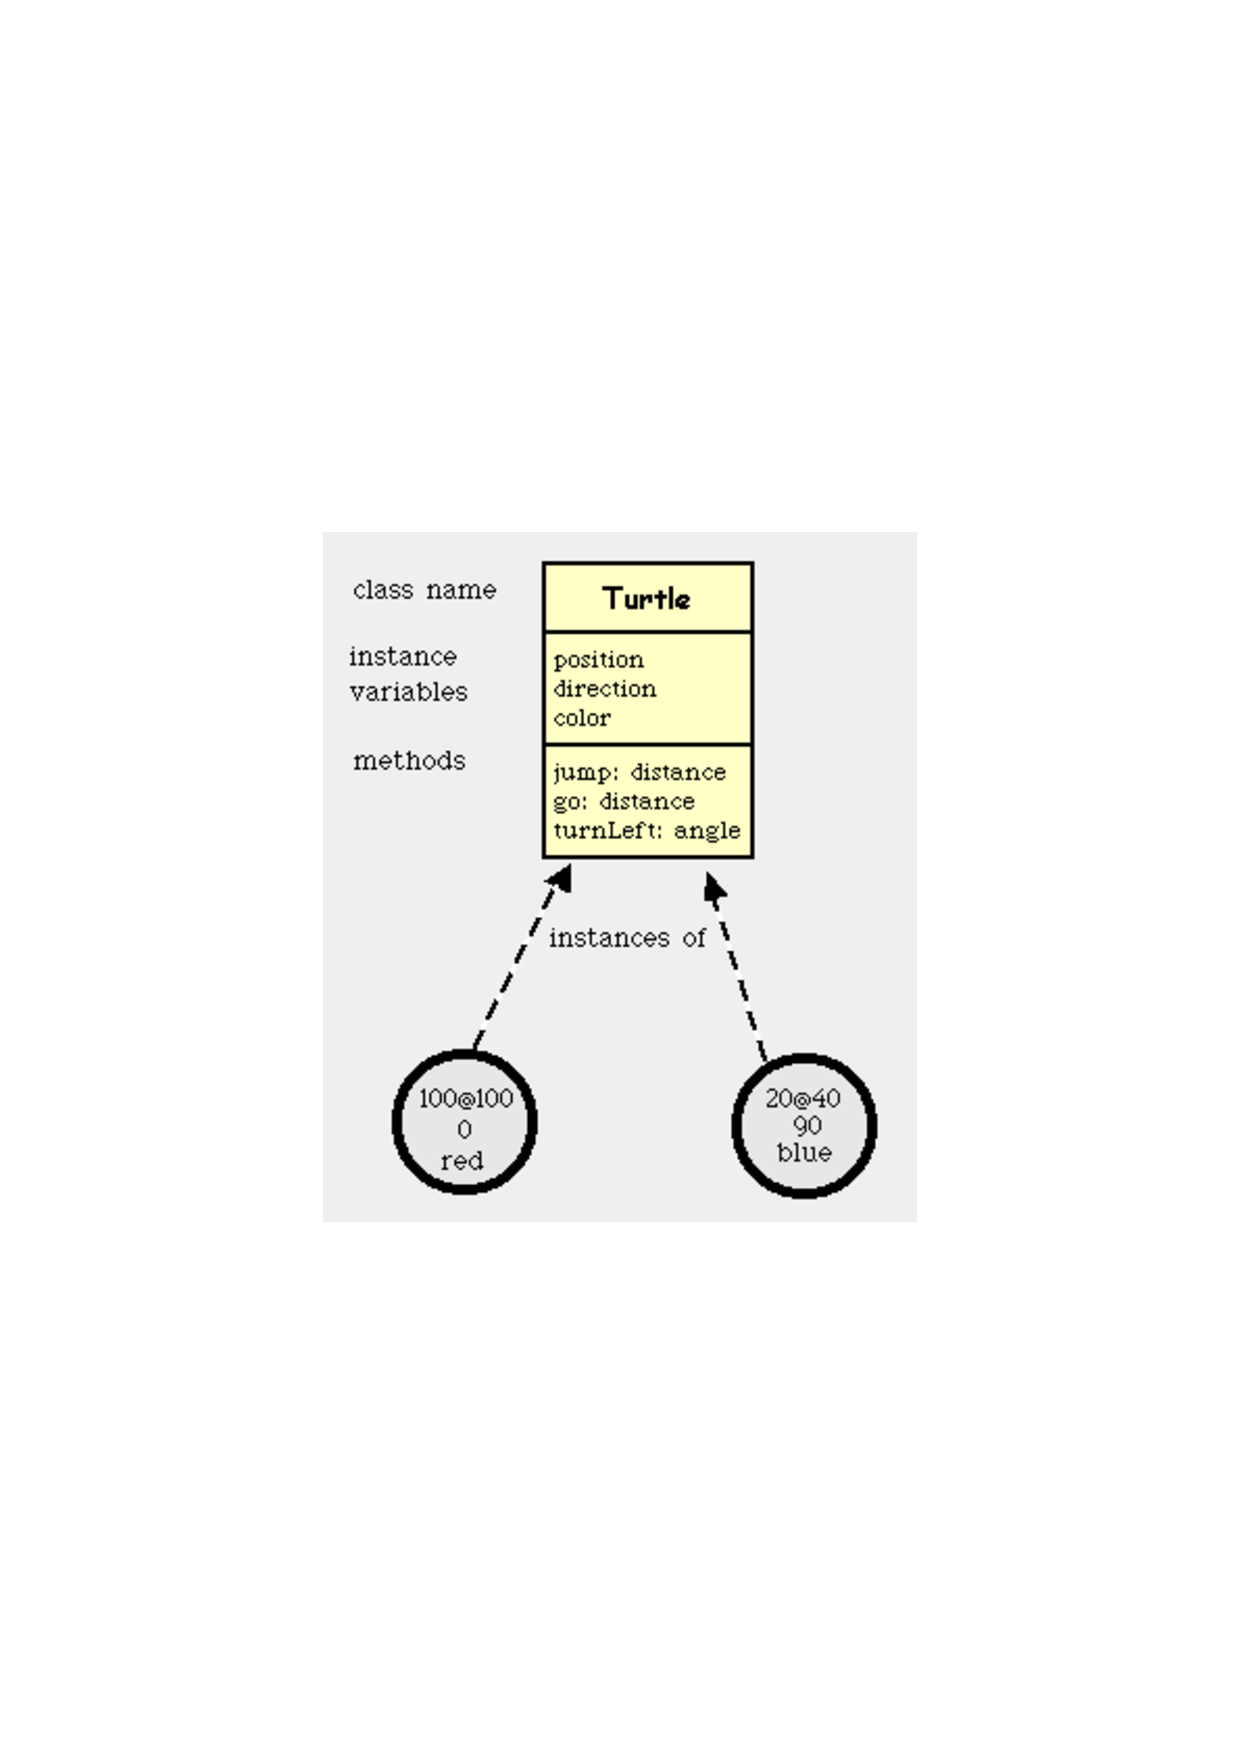
\includegraphics[width=0.5\textwidth]{/Users/ducasse/Workspace/FirstCircle/MyBooks/Bk-Writing/PharoBooks/LearningOOPWithPharoTrans/_result/pdf/Chapters/ObjectsAndClasses/figures/classAndInstances.pdf}\caption{The class \textcode{Turtle} in the UML notation is described by a name, a list of instance variables, and the methods it implements. The instance variables describe the state of the two instances. The instances of a class may have different internal states but share the same interface. They answer the same set of messages..\label{fig:classAndInstances}}\end{center}
\end{figure}



\begin{figure}

\begin{center}
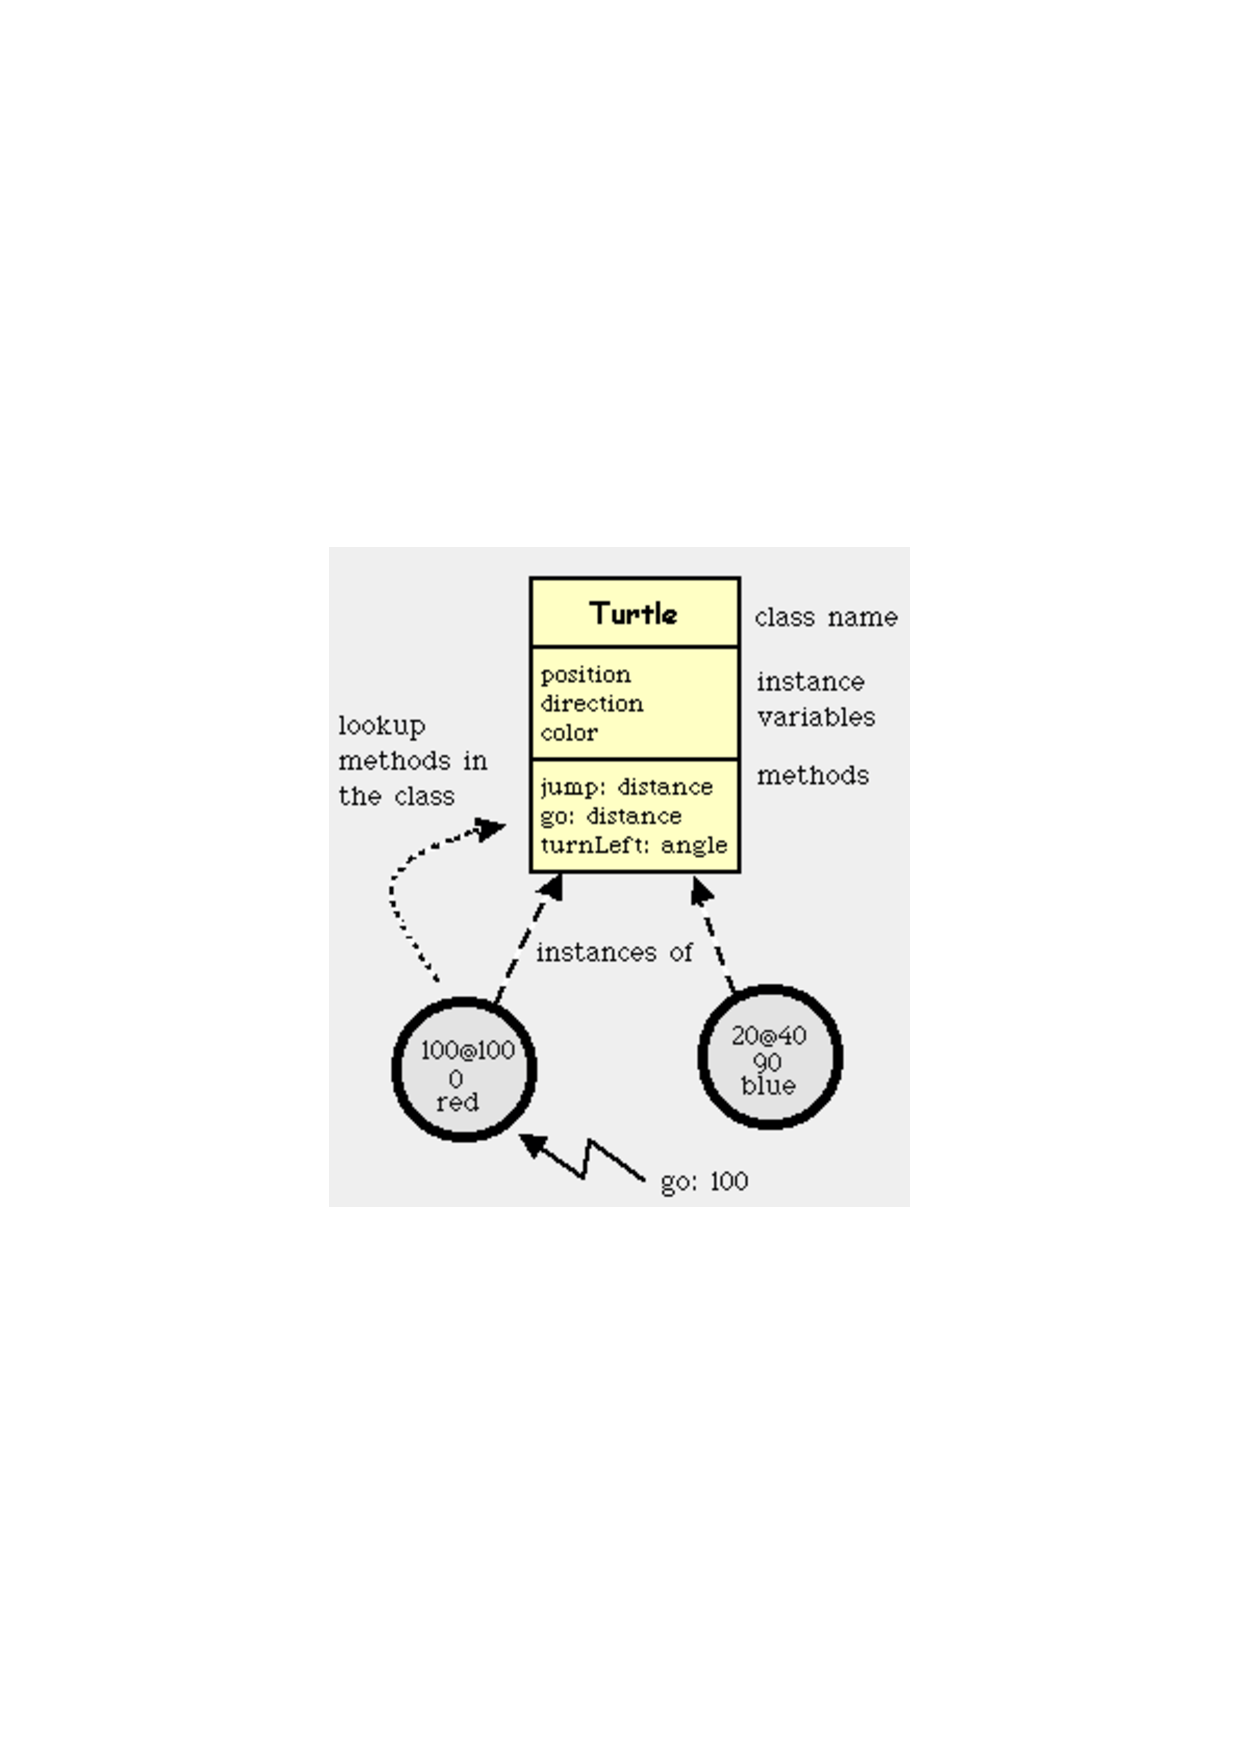
\includegraphics[width=0.5\textwidth]{/Users/ducasse/Workspace/FirstCircle/MyBooks/Bk-Writing/PharoBooks/LearningOOPWithPharoTrans/_result/pdf/Chapters/ObjectsAndClasses/figures/classAndInstancesAndLookup.pdf}\caption{When a message is sent to an object, the corresponding method is looked up in its class. The fine dashed line represents the lookup of the method that goes from the receiver to its class.\label{fig:classAndInstancesAndLookup}}\end{center}
\end{figure}


\begin{important}
Methods define the behavior of all the instances of the class they belong to.
\end{important}
\section{Describing object state}
In addition of being a recipient for object behavior, classes acts as
factory of similar objects. Indeed, \textcode{caro} and \textcode{marg} are both instances of the class \textcode{Turtle} and they
both have a position, a direction, and a color. The class \textcode{Turtle} describes the common internal state of all the turtles.

A class specifies the instance internal state by means of \textit{instance variables}. Instance variables are the variables that each individual instance of the class has and whose \textit{values} represent the state of that instance.

In the definition, the class \textcode{Turtle} defines three instance variables: \textcode{direction}, \textcode{position}, and \textcode{color}. These three instance variables fully describe one of our turtle. We will explain later the first line of the definition but it means that this class specializes the behavior of a class named \textcode{Object} (which defines the default behavior of all objects).

\begin{displaycode}{plain}
Object subclass: #Turtle
	instanceVariableNames: 'direction position color'
	...
    package:: 'Caro-Turtle'
\end{displaycode}

In the sentence \textit{A class describes the internal structure of all its instances}  we would like to stress the fact that the class does not define the state of its instances, it just \textit{describes} it. Hence, any instance can have different values associated with the same instance variables. \textcode{caro} and \textcode{marg} both have a direction instance variable as specified by the class \textcode{Turtle} but they both can have different value associated with it. Hence \textcode{caro}'s direction may be 90 while \textcode{marg}'s direction may be 0 as shown in Figure .

\begin{itemize}
\item All the instances understand the emph\{same\} messages.  One single instance cannot have a specific method.  \textcode{caro} cannot understand a method that \textcode{marg} could not. 
\item All the instances of a class  are represented by the same internal structure which is described in terms of  instance variables, 
\item but instances have different and independent states, i.e., the  values of the instance variables that represent them change from instance of instance. \textcode{caro} can be at a different position than \textcode{marg}.
\end{itemize}

\begin{important}
A class \textit{describes} the internal structure of all its instances by means of instance variables.
\end{important}

Instance variables are special variables that can be accessed from within method body. One of the differences is that they do not need to be declared in the method.  In fact, they are declared in the class definition.  Contrary to  the variables used in scripts, named temporary variables, which do not exist after the script execution, instance variables last as long as the instance does.  

For example, the method \textcode{turn:} needs to increment the receiver's direction by the value of method argument. This is what the method \textcode{turn:} does, it accesses the current value of the instance variable \textcode{direction} and change its value by adding it the method argument.

\begin{displaycode}{plain}
Turtle >> turn: degrees 
   "Change the direction so that the receiver turns by an amount 
   equal to the argument, degrees. degrees represents the rotation in 
   degrees. The positive sense is nonclockwise. The negative sense is 
   clockwise."

   direction := direction + anInteger.
   self changed
\end{displaycode}

The method \textcode{turn:} illustrates that instance variables are accessible from all the methods of the class they belongs to. 
In Pharo, instance variables cannot be accessed from outside of an object. Instance variables are only accessible from the methods of the class that define them. As any other variables instance variables have to be initialized.  This instance variable initialization occurs just after creating a new instance, we will see that in the following chapters.  

\begin{important}
Instance variables are accessible by all the methods of a class. Instance variables have the same lifetime than the object to which they belong to.
\end{important}

\begin{important}
In Pharo, instance variables cannot be accessed from outside of an object. Instance variables are only accessible from the methods of the class that define them.
\end{important}
\section{Class and instances are different}
Classes and objects are different objects; they understand different messages. A class is a factory of objects. A class creates instances.

For example, sending \textcode{new} to the \textcode{Turtle} class returns a newly created turtle, while sending \textcode{new} to a turtle results in an error. In the opposite way, sending \textcode{jump:} to \textcode{Turtle} leads also to an error because \textcode{Turtle} is a factory of objects not the objects themselves. Classes are molders of objects.

\begin{important}
A class describes the state (instance variables) and the behavior (methods) of \textit{all} its instances. The state of an instance is the value of its instance variables and it is specific to one single object while the behavior is shared by all the instances of a class.
\end{important}
\section{Objects reacting differently to the same messages}
Different objects can react in different manner to the same messages.  For example, an animated turtle understands the same messages than a basic turtle. However, it reacts differently to the same message (See\textasciitilde{}ref\{scr:ani\}). An animated turtle performs extra actions related to its animation. Having different behaviors associated with the same message, behavior that  depends on the message receiver is called index\{polymorphism\} emph\{polymorphism\} which literally means multiple form. Polymorphism is a key feature of object-oriented programming languages, it describes that a same message may lead to different method execution depending on the message receiver.

\begin{important}
We send one message but there is probably many methods with the same name. The message passing mechanism will select the
\end{important}

correct method for us. 

\begin{displaycode}{plain}
| caro |
caro := AnimatedTurtle new.
caro go: 100.
caro turnLeft: 90
\end{displaycode}

\begin{displaycode}{plain}
| caro |
caro := Turtle new.
caro go: 100.
caro turnLeft: 90
\end{displaycode}

\begin{important}
Different objects, instances of different classes, can react differently to the same messages.
\end{important}

In the context of \textcode{Turtle} and \textcode{AnimatedTurtle} objects the method execution results in similar, yet different, actions. The receiver gets at the same location in the same state but does extra action i.e., the animation for the animated turtle.  It may happen that different objects understand the same message while doing completely different actions, but this is rare.  

Most of the time it is better to give similar name to methods performing similar behavior, and different names when the methods are doing semantically different actions, so that users of the objects are not confused. As two different classes can define different methods with the same name, it may be confusing for the reader to clearly identify the class to which a method belongs to. Such an issue does not occur when we use the Pharo code browser because a method is always shown in the context of its class. In this book we prefix the method selector with the name of the class and \textcode{ \textgreater{}\textgreater{}}. Hence the method \textcode{square:} defined in the class \textcode{Turtle} is written as follow: 

\begin{displaycode}{plain}
Turtle >> square: anInteger
   "make the receiver draw a square of size anInteger"

   4 timesRepeat: [ self go: anInteger. 
                   self turnLeft: 90 ]
\end{displaycode}

The  polymorphism is really a strength of object-oriented languages because it allows one to treat different objects, i.e., instances of different classes, uniformly as soon as they implement the same messages. Polymorphism works in synergy with the idea that an object is responsible to decide how to react to message reception. Indeed, the fact that different objects can implement the same messages let us write code that only tell the objects to execute some actions without worrying exactly about the kind of objects. 
\subsection{Sending a message vs. calling a method}
The word “method” was introduced in Smalltalk as a metaphor - You tell objects to do something by sending them a message; the object then chooses the method it will use to handle that message.

If you talk about “calling a method” you are breaking the metaphor - it makes no sense in English to “call someone’s method”!
The point is that objects should encapsulate their behavior; you speak to their interface by sending a message. The method is internal – you should not know it.
\section{Conclusion }
\begin{itemize}
\item An object is a computer entity that once created receives messages and performs some actions in reaction.
\item An object has an unique identity.
\item An object holds some private data that represent its internal state.
\item All objects of the same class share the same behavior, i.e., the same method definitions.
\item A class \textit{describes} the internal structure of all its instances by means of instance variable.
\item Instance variables are accessible by all the methods of a class. Instance variables have the same lifetime than the object to which they belong to.
\item In Pharo , instance variables cannot be accessed from outside of an object. Instance variables are only accessible from the methods of the class that define them.
\item A class describes the state (instance variables) and the behavior (methods) of all its instances. The state of an instance is the value of its instance variables and it is specific to one single object while the behavior is shared by all the instances of a class.
\item Methods define the behavior of all the instances  of the class they belong to.
\item Different objects, instances of different classes, can react differently to the same messages.
\end{itemize}


% lulu requires an empty page at the end. That's why I'm using
% \backmatter here.
\backmatter

% Index would go here
\bibliographystyle{abbrv}
\bibliography{others.bib}
\end{document}
